%%%%%%%%%%%%%%%%%%%%%%%%%%%%%%%%%%%%%%%%%%%%%%%%%%%%%%%%%%%%%%%%%%
%%%%%%%%%%%%%%%%%%%%%%%%%%%%%%%%%%%%%%%%%%%%%%%%%%%%%%%%%%%%%%%%%%
% \setmathfont{TeX Gyre Termes Math}
%Packages
\documentclass[10pt, a4paper]{article}
\usepackage[top=3cm, bottom=4cm, left=2cm, right=2cm]{geometry}
\usepackage{amsmath,amsthm,amsfonts,amssymb,amscd, fancyhdr, color, comment, graphicx, environ}
\usepackage{float}
\usepackage{booktabs}
\usepackage{pifont}
\usepackage{mathrsfs}
\usepackage[math-style=ISO]{unicode-math}
\usepackage{lastpage}
\usepackage[dvipsnames]{xcolor}
\usepackage[framemethod=TikZ]{mdframed}
\usepackage{enumerate}
\usepackage[shortlabels]{enumitem}
\usepackage{fancyhdr}
\usepackage{indentfirst}
\usepackage{listings}
\usepackage{sectsty}
\usepackage{thmtools}
\usepackage{shadethm}
\usepackage{hyperref}
\usepackage{setspace}
\usepackage{adjustbox}
\hypersetup{
	colorlinks=true,
	linkcolor=blue,
	filecolor=magenta,
	urlcolor=blue,
}
\usepackage{xcolor,colortbl}
%%%%%%%%%%%%%%%%%%%%%%%%%%%%%%%%%%%%%%%%%%%%%%%%%%%%%%%%%%%%%%%%%%
%%%%%%%%%%%%%%%%%%%%%%%%%%%%%%%%%%%%%%%%%%%%%%%%%%%%%%%%%%%%%%%%%%
%Environment setup
\mdfsetup{skipabove=\topskip,skipbelow=\topskip}
\newrobustcmd\ExampleText{%
	An \textit{inhomogeneous linear} differential equation has the form
	\begin{align}
		L[v ] = f,
	\end{align}
	where $L$ is a linear differential operator, $v$ is the dependent
	variable, and $f$ is a given non−zero function of the independent
	variables alone.
}
\mdfdefinestyle{theoremstyle}{%
	linecolor=black,linewidth=1pt,%
	frametitlerule=true,%
	frametitlebackgroundcolor=gray!20,
	innertopmargin=\topskip,
}
\mdtheorem[style=theoremstyle]{Problem}{Question Number}
\setcounter{Problem}{3}
\newenvironment{Solution}{\textbf{Solution.}}

\definecolor{codegreen}{rgb}{0,0.6,0}
\definecolor{codegray}{rgb}{0.5,0.5,0.5}
\definecolor{codepurple}{rgb}{0.58,0,0.82}
\definecolor{backcolour}{rgb}{0.95,0.95,0.92}

\lstdefinestyle{mystyle}{
	backgroundcolor=\color{backcolour},
	commentstyle=\color{codegreen},
	keywordstyle=\color{magenta},
	numberstyle=\tiny\color{codegray},
	stringstyle=\color{codepurple},
	basicstyle=\ttfamily\footnotesize,
	breakatwhitespace=false,
	breaklines=true,
	captionpos=b,
	keepspaces=true,
	numbers=left,
	numbersep=5pt,
	showspaces=false,
	showstringspaces=false,
	showtabs=false,
	tabsize=2
}

\lstset{style=mystyle}
%%%%%%%%%%%%%%%%%%%%%%%%%%%%%%%%%%%%%%%%%%%%%%%%%%%%%%%%%%%%%%%%%%
%%%%%%%%%%%%%%%%%%%%%%%%%%%%%%%%%%%%%%%%%%%%%%%%%%%%%%%%%%%%%%%%%%
%Fill in the appropriate information below
\newcommand{\norm}[1]{\left\lVert#1\right\rVert}
\newcommand\course{XXXX0000}                            % <-- course name   
\newcommand\hwnumber{0}                                 % <-- homework number
\newcommand\Information{Someone}                        % <-- personal information
%%%%%%%%%%%%%%%%%%%%%%%%%%%%%%%%%%%%%%%%%%%%%%%%%%%%%%%%%%%%%%%%%%
%%%%%%%%%%%%%%%%%%%%%%%%%%%%%%%%%%%%%%%%%%%%%%%%%%%%%%%%%%%%%%%%%%
%Page setup
\pagestyle{fancy}
\headheight 35pt
\lhead{\today \hspace*{4cm} Key-Breakers}
\rhead{
\includegraphics[width=1.2cm]{../logo.png}}
\lfoot{}
\pagenumbering{arabic}
\cfoot{\small\thepage}
\rfoot{}
\headsep 1.2em
\renewcommand{\baselinestretch}{1.25}
%%%%%%%%%%%%%%%%%%%%%%%%%%%%%%%%%%%%%%%%%%%%%%%%%%%%%%%%%%%%%%%%%%
%%%%%%%%%%%%%%%%%%%%%%%%%%%%%%%%%%%%%%%%%%%%%%%%%%%%%%%%%%%%%%%%%%
%Add new commands here
\renewcommand{\labelenumi}{\alph{enumi})}
\newcommand{\Z}{\mathbb Z}
\newcommand{\R}{\mathbb R}
\newcommand{\Q}{\mathbb Q}
\newcommand{\NN}{\mathbb N}
\newcommand{\PP}{\mathbb P}
\DeclareMathOperator{\Mod}{Mod}
\renewcommand\lstlistingname{Algorithm}
\renewcommand\lstlistlistingname{Algorithms}
\def\lstlistingautorefname{Alg.}
\newtheorem*{theorem}{Theorem}
\newtheorem*{lemma}{Lemma}
\newtheorem{case}{Case}
\newcommand{\assign}{:=}
\newcommand{\infixiff}{\text{ iff }}
\newcommand{\nobracket}{}
\newcommand{\backassign}{=:}
\newcommand{\tmmathbf}[1]{\ensuremath{\boldsymbol{#1}}}
\newcommand{\tmop}[1]{\ensuremath{\operatorname{#1}}}
\newcommand{\tmtextbf}[1]{\text{{\bfseries{#1}}}}
\newcommand{\tmtextit}[1]{\text{{\itshape{#1}}}}

\newenvironment{itemizedot}{
	\begin{itemize}
		\renewcommand{\labelitemi}{$\bullet$}
		\renewcommand{\labelitemii}{$\bullet$}
		\renewcommand{\labelitemiii}{$\bullet$}
		\renewcommand{\labelitemiv}{$\bullet$}}
		{\end{itemize}}

\catcode`\<=\active\def<{
\fontencoding{T1}\selectfont\symbol{60}\fontencoding{\encodingdefault}}
\catcode`\>=\active\def>{
\fontencoding{T1}\selectfont\symbol{62}\fontencoding{\encodingdefault}}
\catcode`\<=\active\def<{
\fontencoding{T1}\selectfont\symbol{60}\fontencoding{\encodingdefault}}

%%%%%%%%%%%%%%%%%%%%%%%%%%%%%%%%%%%%%%%%%%%%%%%%%%%%%%%%%%%%%%%%%%
%%%%%%%%%%%%%%%%%%%%%%%%%%%%%%%%%%%%%%%%%%%%%%%%%%%%%%%%%%%%%%%%%%
%Begin now!



\begin{document}
%%%%%%%%%%%%%%%%%%%%%%%%%%%%%%%%%%%%%%%%%%%%%%%%%%%%%%%%%%%%%%%%%%
%%%%%%%%%%%%%%%%%%%%%%%%%%%%%%%%%%%%%%%%%%%%%%%%%%%%%%%%%%%%%%%%%%
%Start the assignment now
%%%%%%%%%%%%%%%%%%%%%%%%%%%%%%%%%%%%%%%%%%%%%%%%%%%%%%%%%%%%%%%%%%
%New problem
\newpage
\begin{Problem}
	\begin{itemize}
		\item Consider that there are two rounds of AES
		      \begin{itemize}
			      \item Using openssl generate a 128-bit message to initialize the AES state matrix.
			      \item Now modify any byte of this state to get another state.
			      \item Run two rounds of AES on these states
			      \item For rounds keys you can use output of Problem-3
			      \item After every operation take the XOR of the states
			      \item In the main assignment show the two states used. Then show how the XOR of the
			            states propagates though each step of the round.
			      \item Verify if you can observe a distinguishing pattern in the output.
			      \item Write a code for the above.
		      \end{itemize}
		\item Also see how the pattern changes as you change the location of the modified byte for the
		      second state.
	\end{itemize}
\end{Problem}

\begin{Solution}

\textbf{Observations}
\begin{itemize}
\item \textbf{Output}

To get output for observation of xor variation run the python file named as
\texttt{AES\_2Round.py} this will dump the output in termial. Ouput will  be as
follows
\begin{center}
	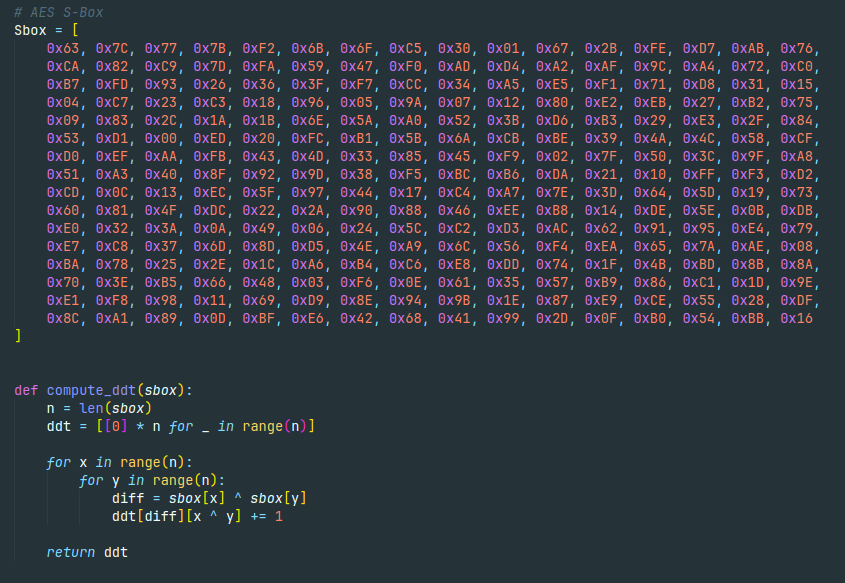
\includegraphics[width=10cm]{p1.png}
\end{center}

\pagebreak
\item \textbf{Distinguishing Pattern}
\begin{itemize}
	\item In message pair only one byte is different, So only byte is not zero in xor diff.

	      \fbox{00000000ed0000000000000000000000}
	\item In Row Shift Operation Xor diff is shifted by some position
	      \begin{center}
		      \text{diff before shifting}
		      \fbox{00000000005e00000000000000000000}

		      \text{diff after shifting }
		      \fbox{000000005e0000000000000000000000}
	      \end{center}
	\item In Mix column diff increases in more positions, than previous one
	      \begin{center}
		      \text{diff before mix column}
		      \fbox{000000005e0000000000000000000000}

		      \text{ diff after mix column}
		      \fbox{  e2000000bc0000005e0000005e000000}
	      \end{center}
	\item Diff in Operation like state xor with key and
	      Substitution diff not changes it is same as previous diff
\end{itemize}

\subsection*{1. Verifying a Distinguishing Pattern in the Output} A
distinguishing pattern is any observable behavior during the AES
transformations (e.g., XOR differences) that allows one to differentiate AES
from a truly random permutation. Based on the implementation and results, the
following observations were made:

\begin{itemize}
	\item The XOR of the ciphertexts consistently has exactly
	      \textbf{4 non-zero bytes} for the given input difference.
	\item The propagation of the XOR difference through the AES transformations
	      (\texttt{SubBytes}, \texttt{ShiftRows}, and \texttt{MixColumns}) shows
	      deterministic behavior, reflecting the structured nature of AES.
	\item Unlike a truly random permutation, which would not produce consistent patterns, AES
	      exhibits predictable propagation of input differences.
\end{itemize}

This deterministic propagation of XOR differences through the AES steps
serves as the \textbf{distinguishing pattern}.

\paragraph{Example:} The following example illustrates the distinguishing
pattern:

\begin{itemize}
	\item \textbf{Messages:}
	      \begin{align*}
		      \text{Message 1:} &
		      \quad \fbox{\texttt{59d0b9515b009b6c69aa9654339a2d8b}} \\
		      \text{Message 2:} & \quad
		      \fbox{\texttt{59d0b9515b009b6c69aa9654339a2dff}}
	      \end{align*}
	\item
	      \textbf{Ciphertexts:}
	      \begin{align*}
		      \text{Cipher 1:} & \quad
		      \fbox{\texttt{992b44622099b43ee6539288017123b6}} \\
		      \text{Cipher 2:} & \quad
		      \fbox{\texttt{c32b44622099b409e653e788012223b6}}
	      \end{align*}
	\item \textbf{XOR of Ciphertexts:}
	      \[
		      \text{Cipher XOR:} \quad
		      \texttt{5a000000000000370000750000530000}
	      \]
	      The XOR difference shows exactly
	      \textbf{4 non-zero bytes}, which is a consistent observation.
\end{itemize}

\paragraph{Propagation of XOR Difference:} The following table illustrates
how the XOR difference propagates through each AES step for the above input:

\begin{table}[H]
	\centering
	\begin{tabular}{|c|c|}
		\hline
		\textbf{Step}                   & \textbf{XOR Difference}                   \\
		\hline
		Message XOR                     & \texttt{00000000000000000000000000000074} \\
		Round Key Apply                 & \texttt{00000000000000000000000000000074} \\
		First Round \texttt{SubBytes}   & \texttt{000000000000000000000000000000b9} \\
		First Round \texttt{ShiftRows}  & \texttt{000000000000000000000000b9000000} \\
		First Round \texttt{MixColumns} & \texttt{b9000000b9000000d000000069000000} \\
		First Round Key Apply           & \texttt{b9000000b9000000d000000069000000} \\
		Second Round \texttt{SubBytes}  & \texttt{5a000000370000007500000053000000} \\
		Second Round \texttt{ShiftRows} & \texttt{5a000000000000370000750000530000} \\
		Second Round Key Apply          & \texttt{5a000000000000370000750000530000} \\
		CipherText                      & \texttt{5a000000000000370000750000530000} \\
		\hline
	\end{tabular}
	\caption{Propagation of XOR Difference Through Each AES Step}
\end{table}

\subsection*{2. How the Pattern Changes with Modified Byte Location} When
the location of the modified byte in the second input message is changed, the
propagation of the XOR difference changes as follows:

\begin{itemize}
	\item The positions of the non-zero XOR bytes in the
	      ciphertext vary based on the modified byte's location in the input.
	\item During the \texttt{ShiftRows} step, the XOR difference is shifted to
	      different positions based on the row-wise shifts.
	\item During the
	      \texttt{MixColumns} step (first round only), the XOR difference spreads to
	      multiple bytes within the same column, resulting in more non-zero bytes in
	      the XOR.
\end{itemize}

\paragraph{Empirical Observations:} For example, modifying the byte at
position \texttt{(3, 3)} in the input message produced the following results:

\begin{itemize}
	\item \textbf{Ciphertext XOR:} \[ \text{Cipher XOR:} \quad
		      \texttt{5a000000000000370000750000530000} \] The XOR difference has \textbf{4
		      non-zero bytes} at fixed positions: \texttt{(0, 1)}, \texttt{(14, 15)},
	      \texttt{(20, 21)}, \texttt{(26, 27)}.
	\item When the modified byte is moved to position \texttt{(2, 2)}, the
	      non-zero XOR bytes in the ciphertext appear at different positions but
	      follow the same deterministic propagation pattern.
\end{itemize}
\end{Solution}

%%%%%%%%%%%%%%%%%%%%%%%%%%%%%%%%%%%%%%%%%%%%%%%%%%%%%%%%%%%%%%%%%%
%Complete the assignment now
\end{document}

%%%%%%%%%%%%%%%%%%%%%%%%%%%%%%%%%%%%%%%%%%%%%%%%%%%%%%%%%%%%%%%%%%
%%%%%%%%%%%%%%%%%%%%%%%%%%%%%%%%%%%%%%%%%%%%%%%%%%%%%%%%%%%%%%%%%%
